
\chapter{Anforderungen an die Web Applikation}

\section{Spot Beschreibungen}

Eine der bekanntesten Wellen in Europa ist im spanischen Baskenland an
einer Fluss\-mündung östlich des Ortes \textit{Mundaka} zu finden. Im
\textit{Stormrider Guide Europe} \cite[S.180]{storm_europe_1998}
werden die Surfbedingungen an diesem Spot wie folgt beschrieben.

\textit{Some of the longest, hollowest lefts in Europe break over
  sandbanks at the mouth of the river Gernike. It's best at low tide,
  when the rivers current (a useful conveyor belt) is less intense,
  and holds swell up to 4m (12ft). On the other side of the rivermouth
  are the beaches Laida and Laga where you can find waves at small
  swells. The river and its estuary are a Worldwide Fund for Nature
  reserve, but even so, the water is not as clean as could expected.
}

Zusätzlich werden den Beschreibungen Piktogramme aus verschiedenen
Kategorien zugeordnet, welche die Gegebenheiten vor Ort durch eine
vereinfachte grafische Darstellung widerspiegeln. Einige dieser
Kategorien sind die bevorzugte Windrichtung, die optimale Gezeit, die
Art der brechenden Welle, Beschaffenheit des Bodens, sowie mögliche
Gefahren. Kennt man einmal die Piktogramme, ist durch einen kurzen
Blick schnell ersichtlich welche Bedingungen an einem Spot herrschen.

\begin{figure}[h]
  \begin{center}
    
\includegraphics[height=40px]{bilder/mundaka-conditions}
    \caption{Piktogramme zu den Surfbedingungen in Mundaka}
    \label{piktogramm}
  \end{center}
\end{figure}

In Abbildung \ref{piktogramm} sind die Piktogramme zu sehen, die für
die obige Beschreibung in Mundaka verwendet wurden. Sie sollen
vermitteln, dass dieser Spot sehr bekannt ist und an guten Tagen mit
vielen Surfern zu rechnen ist. Die Welle bricht mit viel Kraft von
links nach rechts (\textit{Left-hander}, immer vom Strand aus gesehen)
über einer Sandbank, wobei vereinzelt Surfbretter zu Bruch gehen
können.  Sie ist nicht bei Flut (\textit{High Tide}) surfbar, und
ablandiger Wind (\textit{Offshore}) aus dem Süden trägt dazu bei, dass
die Wellen geglättet werden, später brechen und hohler werden.

Das Konzept der Stormrider Guides soll die Grundlage der Web
Applikation bilden und mit den neuen Möglichkeiten des Internets
verknüpft werden. Die Beschreibungen zu den Spots und deren
Gegebenheiten sollen gemeinschaflich durch die Mitglieder der Surf
Community verfasst werden, und als sogenannter \textit{User Generated
  Content} verwaltet werden. Die gemeinsam erstellten Beschreibungen
sollen eine objektive Sicht auf die Gegebenheiten und Surfbedingungen
an den jeweiligen Spots bieten. Für persönliche Ansichten und
Diskussionen sollen Kommentarfunktionen zur Verfügung gestellt werden
die in Abschnitt \ref{subsec:Kommentare} beschrieben werden.

Um Spam und anderer mutwilliger Zerstörung oder Verunreinigung des
Contents vorzubeugen ist eine Registrierung der Nutzer
erforderlich. Für alle Informationen die zu einem Spot gehören und von
Nutzern der Web Applikation verändert werden können, soll eine
Historie verwaltet werden. Dies soll sicherstellen, dass bei einer
eventuellen Veruneinigung des Contents auf eine frührere Version der
Information zurückgegriffen, und diese wiederhergestellt werden kann.

\section{Kartenmaterial}

Um das Auffinden von Spots zu vereinfachen sollen diese auf einer
Karte dargestellt werden. Webservice Dienste wie \textit{Google Maps},
\textit{Yahoo! Maps} oder Microsoft's \textit{Bing Maps}
\footnote{seit Juni 2009, früher: Microsoft's Virtual Earth} bieten
die Möglichkeit interaktive Karten per Java\-script oder Flash in eine
Webseite einzubetten. Diese Dienste bieten nicht nur die typischen
Land- bzw. Straßenkarten an, sondern stellen auch Satelitenbilder und
teilweise 3-dimensionale Ansichten für bestimmte Gebiete zur
Verfügung.

\begin{figure}[h]
  \subfigure[Karten Ansicht]{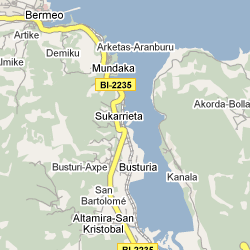
\includegraphics[width=0.49\textwidth]{bilder/google-maps-map}}
  \subfigure[Satelliten Ansicht]{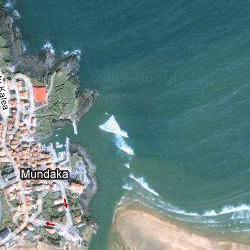
\includegraphics[width=0.49\textwidth]{bilder/google-maps-hybrid}}
  \caption{Google Maps Kartenmaterial für Mundaka, Spanien}
\end{figure}

\section{Wetter- und Wellendaten}
\label{sec:Wetter- und Wellendaten}

Wie schon in der Einleitung erwähnt ist das Vorhandensein von Swell
eine der Grundvoraussetzungen zum Surfen. Viele Surfer nutzen deshalb
regelmäßig Dienste im Internet um sich über die Wetter- und
Wellenverhältnisse in den nächsten Tagen zu informieren. Dabei ist
hauptsächlich die Wellenhöhe, die Wellenperiode und die Stärke und
Richtung des Windes von Interesse. Die Spot Beschreibungen sollen
deshalb mit aktuellen Wetter- und Wellenvorhersagen verknüpft werden,
um den Benutzern der Web Applikation einen Mehrwert zu bieten. Die
\textit{National Oceanic and Atmospheric Administration (NOAA)} ist
die Wetter- und Ozeanografiebehörde der Vereinigten Staaten. Sie
besteht aus 5 größeren Organisationen, zu denen unter anderen auch der
\textit{National Weather Service} und der \textit{National Ocean
  Service} gehören, welche die benötigten Wetter- und Wellendaten zur
Verfügung stellen. Viele der im Internet verfügbaren Dienste, die
Wetter- oder Wellenvorhersagen anbieten, beziehen ihre Daten ebenfalls
von diesen Organisationen.

\section{Bilder \& Videos}

Um Surfern einen visuellen Eindruck von einem Spot zu bieten, sollen
die Spots mit Bildern und Videos verknüpft und somit aufgewertet
werden. Auf Internetseiten wie \textit{Flickr} und \textit{YouTube}
sind von vielen bekannten Spots Bilder und Videos zu finden. Eine
Suchanfrage nach einem der bekanntesten Spots mit den Stichwörtern
\textit{Mavericks} und \textit{Surf} ergab im Juni 2009 bei
\textit{Flickr} 2319 und bei \textit{YouTube} 548 Ergebnisse. Diese in
der Surf Community gerne gesehenen Bilder und Videos sind ideal um das
bisher aus Beschreibungen und Wetter-/Wellenvorhersagen bestehende
Informationsangebot zu erweitern. Sowohl \textit{Flickr} als auch
\textit{YouTube} bieten eine Webservice Schnittstelle an, mit der es
möglich ist deren Bilder und Videos in eigene Anwendungen zu
integrieren. Zudem soll den Nutzern die Möglichkeit gegeben werden
ihre eigenen Bilder und Videos auf die Community Plattform zu laden
und dort zu veröffentlichen.

\begin{figure}[h]
  \begin{center}
    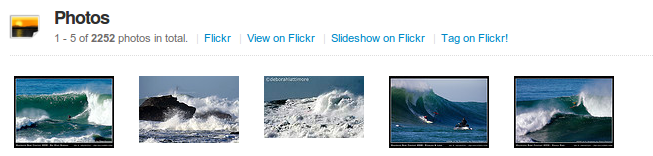
\includegraphics[width=\textwidth]{bilder/photos-flickr}
    \caption{Integration von Bildern durch den Flickr Webservice}
    \label{piktogramm}
  \end{center}
\end{figure}

\begin{figure}[h]
  \begin{center}
    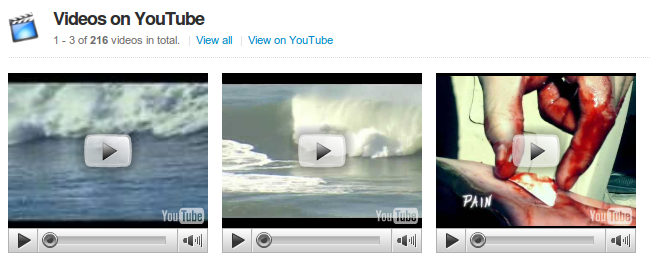
\includegraphics[width=\textwidth]{bilder/videos-youtube}
    \caption{Integration von Videos durch den YouTube Webservice}
    \label{piktogramm}
  \end{center}
\end{figure}

\section{Community Funktionen}

Einige Funktionen, die aus Community Plattformen wie \textit{Facebook}
und \textit{StudiVZ} bekannt sind sollen auch in dieser Web
Applikation zu Verfügung stehen. Ziel ist auch hier einen Mehrwert für
die Nutzer zu generieren, um diese näher an die Plattform zu binden.

\subsection{Freundschaften}
Nutzer sollen in der Lage sein Freundschaftsanfragen an andere Nutzer
zu stellen, und Anfragen anderer Nutzern zu akzeptieren
bzw. abzulehnen.

\subsection{Nachrichten}

\subsection{Kommentare}
\label{subsec:Kommentare}

Spot Beschreibungen sollen eine objektive Sicht auf die


\subsection{Secret Spots}

%%% Local Variables:
%%% mode: latex
%%% TeX-master: "../community-plattform"
%%% End:
